\documentclass[10pt]{beamer}

\usecolortheme{dove}
\definecolor{mycyan}{rgb}{0.2157, 0.7059, 0.9608}
\setbeamercolor{alerted text}{fg=mycyan}
\setbeamertemplate{bibliography item}{\insertbiblabel}
\setbeamertemplate{caption}[numbered]
\hypersetup{colorlinks,linkcolor=,urlcolor=mycyan}
\usepackage{animate,xcolor,colortbl,listings,nicefrac}
\usepackage[italian]{babel}

\usepackage{listings}
\lstset{upquote=false}
\usepackage[]{framed}
\begin{document}


\begin{frame}
  \title{Metodi di Krylov}
  \subtitle{Metodi per la soluzione numerica di equazioni lineari non simmetriche applicabili in un sottospazio di Krylov.}
  \date{29/04/2020}
  \author[Principal]{Fabio Archenti \and Fabio Camagni \and Andrea Favero \and  \\Lorenzo Fiamingo \and Stefano Gallivanone \and Nazariy Nashkolnyy}
  \maketitle
\end{frame}


\begin{frame}
    \frametitle{Bibliografia}
    
  \begin{thebibliography}{99}\small
    \bibitem{quarteroni2012calcolo}
    Quarteroni, Saleri, and Gervasio.
    \newblock {\em Calcolo Scientifico: Esercizi e problemi risolti con MATLAB e  Octave}.
    \newblock UNITEXT. Springer Milan, 2012.

    \bibitem{trefethen-bau}
    Trefethen, and Bau.
    \newblock {\em Numerical Linear Algebra}.
    \newblock SIAM, 1997.
    
   
   \bibitem{dac95}
   Telichevesky, Kundert, and White.
   \newblock {\em Efficient Steady-State Analysis based on Matrix-Free Krylov-Subspace Methods}.
   \newblock {\em Scientific report}, June 1995.

   \end{thebibliography}

%Una volta inserito un documento in bibliografia, 
%può essere citato così:~\cite{quarteroni2012calcolo}
  
\end{frame}  

\begin{frame}
  \frametitle{Sommario}
  %Questo comando inserisce una lista delle sezioni in
  %cui è divisa la presentazione. Perché una sezione appaia 
  %nel sommario deve contenere almeno una pagina.
  \tableofcontents
\end{frame}

\section{Introduzione}\label{sec:sec1}

\begin{frame} \frametitle{Introduzione}
\begin{itemize}
    \item I metodi di Krylov sono metodi iterativi utilizzati per risolvere sistemi lineari A$\mathbf{x}=\mathbf{b}$.

    \item Data una matrice A di dimensione $\mathit{n}$ e un vettore $\mathbf{v}\in \mathbb{R}^n$, si definisce \alert{sottospazio di Krylov} lo spazio
    $$
    \mathcal{K}_\mathrm{n}(A,\mathbf{v})=span\{\mathbf{v},A\mathbf{v},A^2\mathbf{v},\dots,A^{n-1}\mathbf{v}\}, n\geq1
    $$

    \item Ad ogni passo dell'iterazione viene calcolata una soluzione approssimata $\mathbf{x}^\mathit{n}$ appartenente al sottospazio di Krylov $\mathcal{K}_\mathrm{n}(A,\mathbf{r}_0)$, dove $\mathbf{r}_0=\mathbf{b}-A\mathbf{x}_0$ è il vettore residuo al passo 0 e $\mathbf{x}_0$ è la soluzione calcolata al passo 0.
    
\end{itemize}
\end{frame}

\section{Metodo del Gradiente Coniugato}\label{sec:sec2}

\begin{frame} \frametitle{Metodo del Gradiente Coniugato (I)}
\begin{itemize}
    \item Data A matrice simmetrica e definita positiva, possiamo definire la funzione (forma quadratica) $\phi:\mathbb{R}^n \to \mathbb{R}$ $$\phi(\mathbf{x})=\frac{1}{2}\mathbf{x}^TA\mathbf{x}-\mathbf{x}^T\mathbf{b}.$$
    
    \item Questa funzione (se le ipotesi su A sono verificate) è una funzione convessa e ammette un unico punto $\mathbf{x}^{\ast}$ di minimo assoluto.
    
    \item $\nabla \phi(\mathbf{x})=A\mathbf{x}-\mathbf{b}$. Nel punto $\mathbf{x}^{\ast}$ il gradiente si annulla:  $\nabla \phi(\mathbf{x}^{\ast})=A\mathbf{x}^{\ast}-\mathbf{b}=\mathbf{0}$.
    Risolvere il problema di minimo (trovando $\mathbf{x}^{\ast}$) equivale quindi a risolvere il sistema A$\mathbf{x}=\mathbf{b}$.

\end{itemize}
\end{frame}

\begin{frame} \frametitle{Metodo del Gradiente Coniugato (II)}
\begin{itemize}
    \item Per minimizzare $\phi(\mathbf{x})$, partendo da una \alert{guess} iniziale $x_0$, dobbiamo scegliere una \alert{direzione di discesa} $\mathbf{d}_{k}$ (ovvero un vettore $\in \mathbb{R}^n$) e un \alert{passo di discesa} $\alpha_k$ (con $\alpha_k \in \mathbb{R}$) ponendo $\mathbf{x}_{k+1}=\mathbf{x}_{k}+\alpha_k\mathbf{d}_{k}$.
    
    \item Scegliamo ad ogni passo una direzione A-ortogonale rispetto a tutte le direzioni precedenti, cioè tale che $(A\mathbf{d}_{j})^T\mathbf{d}_{k+1}=\mathbf{0}$ e $(\mathbf{r}_{k+1})^T\mathbf{d}_j=\mathbf{0}$ $j=0,\dots,k$.
    
    \item All'inizio $\mathbf{d}_0=\mathbf{r}_0$, poi $(\mathbf{d}_{k+1})=\mathbf{r}_{k+1}-\beta_k\mathbf{d}_k$ per $k=0,\dots,n-1$, con $\beta_k=\frac{(A\mathbf{d}_{k})^T\mathbf{r}_{k+1}}{(A\mathbf{d}_{k})^T\mathbf{d}_{k}}$ (scelta ottimale).
    
    \item In questo modo le $\mathbf{d}_k$ sono linearmente indipendenti e la soluzione $\mathbf{x}_{k+1}$ è ottimale rispetto a tutte le direzioni di discesa (ovvero $\mathbf{r}_{k+1}$ è ortogonale a $\mathbf{d}_k$): è garantito che $\mathbf{x}_n=\mathbf{x}^{\ast}$.
\end{itemize}
\end{frame}


\begin{frame} \frametitle{Passo di discesa}
\begin{itemize}
\item Il passo di discesa più convenient è $\alpha=...$
\item Dimostrazione:
\begin{itemize}
    \item La soluzione al passo $k+1$ è $\mathbf{x}_{k+1}=\mathbf{x}_{k}+\alpha_k\mathbf{d}_{k}$
    \item Sostituendo nella forma quadratica
    \end{itemize}

\end{itemize}
\end{frame}

\begin{frame} 
\begin{center}
\begin{tabular}{ c }
\hline\\
\textbf{Generalized Minimal RESidual} \\ [0.5ex]
risoluzione di un sistema lineare tramite sottospazio di Krylov\\ \\
 \hline
\end{tabular}
\end{center}
\end{frame}

\section{GMRES}\label{sec:sec3}

\begin{frame} \frametitle{GMRES}
\begin{itemize}
    \item \textbf{GMRES} (Generalized Minimal RESidual) è uno dei metodi di Krylov utilizzato per risolvere il sistema lineare $Ax = b$ tramite il sottospazio
    $\mathcal{K}_\mathrm{n}$ in modo tale da rendere minima la norma Euclidea del residuo: $$\|\mathbf{b}-A\mathbf{x_n}\|_2.$$
    
    \item Sia $K_n$ la matrice $m x n$ di Krylov, composta da spazi colonne A$\mathcal{K}_\mathrm{n}$. Inanzitutto si moltiplica $K_n$ per A, per cui il problema diventa trovare un vettore $\mathbf{c}\in\mathbb{C}^n$, tale per cui il residuo $\|AK_n\mathbf{c}-\mathbf{b}\|_2$ sia minimo. 
    
    \item Questa formula è risolvibile con fattorizzazione QR, ma $AK_n$ diventa \textbf{numericamente instabile} al crescere di $n$, quindi si utilizza \alert{l'iterazione di Arnoldi} per costruire una base di vettori ortonormali.

\end{itemize}
\end{frame}

\begin{frame} \frametitle{L'iterazione di Arnoldi (I)}
\begin{itemize}
    \item Si definisce $Q_n$ come la matrice, i cui vettori formano una base ortonormale di $\mathcal{K}_\mathrm{n}$. Il problema consiste ora nella ricerca di $\mathbf{y}\in\mathbb{C}^n$ tale per cui: $$\|AQ_n\mathbf{y}-\mathbf{b}\|_2 = minimo,$$ riducendo così le dimensioni del problema da $m x n$ a $(n+1) x n$.
    
    \item L'iterazione di Arnoldi dimostra che $AQ_n = Q_{n+1}\mathcal{H}_n$ (con $\mathcal{H}_n$ la matrice alta-sinistra, $(n+1) x n$, della matrice di Hessenberg). Il problema quindi diventa:$$\|Q_{n+1}\mathcal{H}_n\mathbf{y}-\mathbf{b}\|_2 = minimo.$$ 
\end{itemize}
\end{frame}


\begin{frame} \frametitle{L'iterazione di Arnoldi (II)}
\begin{itemize}
    \item Moltiplicando entrambi i membri per $Q^*_{n+1}$ si ottiene: $$\|\mathcal{H}_n\mathbf{y}-Q^*_{n+1}\mathbf{b}\|_2 = minimo.$$
    \item Si osserva che $Q^*_{n+1}\mathbf{b}=\|\mathbf{b}\|\mathbf{e_1}$, con $\mathbf{e_1}=(1,0,0,\dots)^*$, quindi il problema 
    finale è:$$\|\mathcal{H}_n\mathbf{y}-\|\mathbf{b}\|\mathbf{e_1}\|_2 = minimo.$$ Questa equazione è risolvibile con l'approssimazione ai minimi quadrati.
\end{itemize}


\end{frame}

\begin{frame} 
\begin{center}
\begin{tabular}{ c }
\hline\\
\textbf{Generalized Minimal RESidual} \\ [0.5ex]
applicazione nel calcolo polinomiale\\ \\
 \hline
\end{tabular}
\end{center}
\end{frame}

\begin{frame} \frametitle{GMRES Polinomi}
\begin{itemize}
    \item Il metodo GMRES è utilizzabile anche nel calcolo polinomiale.
    \item Dato $p_n\in P_n$, con $p_n(0)=1$ si definisce $x_n=q_n(A)\mathbf{b}$ e $r_n=p_n(A)\mathbf{b}$. Il problema consiste nel calcolare $p_n\in P_n$ tale che $$\|r_n\|=minimo.$$
\end{itemize}
\end{frame}


\begin{frame} \frametitle{Velocità di convergenza}\framesubtitle{Quanto deve valere \textbf{n} (numero di iterazioni) per soddisfare la tolleranza?}
    $$ \frac{\|r_n\|}{\|\mathbf{b}\|}  < tolleranza$$
\begin{itemize}
    \item Osservazione 1: convergenza monotona $\|r_{n+1}\|\leq \|r_n\|$.
    \item Osservazione 2: per $n\to \infty$, $\|r_{\infty} \|= 0$, a meno di errori di arrotondamento.
    \item Essendo $\|r_n\| = \|p_n(A) \mathbf{b}\| \leq\|p_n(A)\|\|\mathbf{b}\|$ risulta che solo $p_n(A)$ influenza la velocità di convergenza: $$\frac{\|r_n\|}{\|\mathbf{b}\|} \leq inf\|p_n(A)\|,$$ con $p_n \in P_n$.
\end{itemize}
\end{frame}


\begin{frame} 
\begin{center}
\begin{tabular}{ c }
\hline\\
 \textbf{Analisi stazionaria efficiente} \\ [0.5ex]
  \textbf{basata sul metodo matrix-free nei sottospazi di Krylov}\\ \\
 \hline
\end{tabular}
\end{center}
\end{frame}


\begin{frame}
\frametitle{Matrix Free GMRES}\framesubtitle{Esempio applicativo del metodo: \textbf{circuiti analogici}}
\begin{itemize}
\item Più circuiti $\to$ più problemi per risolverli
\item Risposta del circuito dipende dagli ingressi (ampiezze, frequenze) $\to$ migliaia di punti da verificare
\item N equazioni $\to$ $N^3$ flops per Gauss, $N^2$ flops per metodi iterativi
\item Matrix-Free VS Iterativi: se N=400 $t_{It} \approx 10t_{MF}$
\end{itemize}
\end{frame}


\begin{frame}
\frametitle{Matrix Free GMRES}\framesubtitle{Algoritmo per calcolare la distorsione nei circuiti analogici}
%[CANCELLA](cerco stato stazionario periodico = le variabili di stato non dipendono dal tempo)[CANCELLA]
\begin{itemize}
\item I dati si ricavano simulando il circuito e misurando i valori ottenuti in un periodo T.
\begin{equation}
f(\mathbf{v}(t),t) = \mathbf{i}(\mathbf{v}(t)) + \mathbf{q}'(\mathbf{v}(t)) + \mathbf{u}(t) = 0	           
\end{equation}
\footnotetext{$\mathbf{v}$, $\mathbf{i}$, $\mathbf{q}$, $\mathbf{u} \in   \mathbb{R}^N$\\} 
\begin{equation}
\mathbf{v}(T) - \mathbf{v}(0) = 0 
\end{equation}
\item Dalla (1) e (2) si ricava  \begin{equation}
\mathbf{\phi}(\mathbf{v}(0),0,T) - \mathbf{v(0)}
 = 0
 \end{equation}
\item Dove \[ \phi = \int\limits_0^T f(\mathbf{v}(t),t) dt\]
%[CANCELLA](funzione di stato)[CANCELLA] 
\end{itemize}
\end{frame}


\begin{frame}
\frametitle{Matrix Free GMRES}
\framesubtitle{Iterazione di Newton (I)}
\begin{itemize}
\item Tramite il metodo di Newton alla (3) si ottiene l'iterazione\begin{equation}
\mathbf{v}_0^j = \mathbf{v}_0^{j-1} - [J_{\phi}(\mathbf{v}_0^{j-1},0,T) - I]^{-1}[\phi(\mathbf{v}_0^{j-1},0,T) - \mathbf{v}_0^{j-1}]
\end{equation}con $\mathbf{v}_0 = \mathbf{v}(t=0)$.       
\item Utilizzando opportuni passaggi(vedi dac95 paragrafo 2) si ricava la formula
\end{itemize} 
 \begin{equation}
\bigg[\frac{\mathbf{C}(\mathbf{v}_m^{l-1})}{h_m} + \mathbf{G}(\mathbf{v}_m^{l-1})\bigg](\mathbf{v}_m^l-\mathbf{v}_m^{l-1}) = - \frac{1}{h_m}(\mathbf{q}(\mathbf{v}_m^{l-1}) - \mathbf{q}(\mathbf{v}_{m-1})) - \mathbf{i}(\mathbf{v}_m^{l-1}) - \mathbf{u}_m
\tag{8}
\end{equation}
\end{frame}


\begin{frame}
\frametitle{Matrix Free GMRES}
\framesubtitle{Iterazione di Newton (II)}
Siano\\
\begin{itemize}
\item m = instante temporale%[CANCELLA](suddivido T in M instanti)[CANCELLA]
\item $h_m = t_m - t_{m-1}$
\item $\mathbf{C} = \frac{d\mathbf{q}}{d\mathbf{v}}$
\item $\mathbf{G} = \frac{d\mathbf{i}}{d\mathbf{v}}$ 
\item $J_f = \frac{\mathbf{C}(\mathbf{v}_m^{l-1})}{h_m} + \mathbf{G}(\mathbf{v}_m^{l-1})$
\end{itemize}
 La sensibilità si esprime come
 \begin{equation}
J_f(\mathbf{v}_m)\frac{d\mathbf{v}_m}{d\mathbf{v}_0} = \frac{\mathbf{C}(\mathbf{v}_{m-1})}{h_m}\frac{d\mathbf{v}_{m-1}}{d\mathbf{v}_0}
\tag{11}
\end{equation}
L'iterazione di Newton richiede circa $N^2$ flops.\footnote{N = dim($\mathbf{v}$)\\}
\end{frame}

\begin{frame}
\frametitle{Matrix Free GMRES}\framesubtitle{\textbf{Algoritmo (I)}. Per risolvere Ax = b con GMRES}

$\mathbf{x}_0 =$ Guess iniziale\\
$p_0 = b - A\mathbf{x}_0$ (direzione)\\
k = 1\\
do \{\\
$p^k = Ap^{k-1}$ (nuova direzione)\\
$p^k = p^k -\sum\limits_{j=0}^{k-1}\beta_{k,j}p^j$ (ortogonalizza)\\
cerca $\alpha_k$ in $x^k = x^{k -1} + \alpha_kp^k$ tale che\\
$\|r^k\| = \|\mathbf{b} - A\mathbf{x}^k\|$ minimo\\
$k = k + 1$\\
\} while($\|r^k\| < tolerance_{GMRES}$)\\
$\mathbf{x}^k = soluzione$
  
\end{frame}

\begin{frame}
\frametitle{Matrix Free GMRES}
\begin{itemize}
\item Il costo elevato dell'iterazione di Newton è causato dal calcolo di $ A = J_\phi - I$: $dim(A) = N^2$
\item Il GMRES matrix free consente di risolvere il sistema senza memorizzare l'intera matrice A  
%[CANCELLA(il computer memorizza A in forma sparsa,ovvero tiene in memoria solo i valori di A utili al calcolo della soluzione)CANCELLA]
\item 
Così facendo il calcolo di $J_\phi p^{k-1}$ richiede circa N operazioni\footnote{$J_\phi p^{k-1}$ serve a calcolare $Ap^{k-1}$ in ogni step k dell'iterazione \\}
\end{itemize}
\end{frame}


\begin{frame}
\frametitle{Matrix Free GMRES}
\begin{itemize}
\item $Ap^{k-1} = (J_\phi - I)p^{k-1}$ è approssimabile a meno di un errore $\epsilon$ \\\begin{equation} \frac{\phi(\mathbf{v}_0 + \epsilon p^{k-1},0,T) - \phi (\mathbf{v}_0)}{\epsilon} - p^{k-1}
\tag{12}
\end{equation}
%\item [CANCELLA](vedi frase dac 95 sotto la(12))[CANCELLA]
\item L'algoritmo utilizzato per risolvere la (12) richiede lo stesso numero di operazioni necessario a calcolare una sola colonna di $J_\phi$ con il metodo di Newton
\item Salvare $\mathbf{C}(\mathbf{v}_m)$ e fattorizzare LU $J_f(\mathbf{v}_m)$ ad ogni passo per applicare:
\end{itemize}
\begin{equation}
J_f(\mathbf{v}_m)\frac{d\mathbf{v}_m}{d\mathbf{v}_0} = \frac{\mathbf{C}(\mathbf{v}_{m-1})}{h_m}\frac{d\mathbf{v}_{m-1}}{d\mathbf{v}_0}
\tag{11}
\end{equation}  
\end{frame}


\begin{frame}
\frametitle{Matrix Free GMRES}\framesubtitle{\textbf{Algoritmo (II)}. Per risolvere Ax = b matrix free}

$\mathbf{v}_0 =$ Guess iniziale \\
 For j = 1 to Max Newton \{ \\
 $\int\limits_{0}^{T} (1) dt$ con $\mathbf{v}_0 = \mathbf{v}_0^{j-1}$ \\
 For m = 1 to M \{ \\
 Risolvi la (6) \\
 Salva $J_f(\mathbf{v}_m)$ e $\mathbf{C}(\mathbf{v}_m)$ \\
 \}\\
 Risolvi $(J_\phi(\mathbf{v}^{j-1}) - I)\delta\mathbf{v}^j = \mathbf{v}^{j-1} - \phi(\mathbf{v}^{j-1})$ con GMRES\\
 Nel GMRES calcola $p^{k+1} = J_\phi(\mathbf{v}^{j-1})p^k$ usando\\
 $p^{k+1} = p^k$ \\
 For m = 1 to M risolvi $J_f(\mathbf{v}_m)p^{k+1} = \mathbf{C}(\mathbf{v}_{m-1})p^{k+1}$ \\
 
 $\mathbf{v}^j = \mathbf{v}^{j-1} + \delta\mathbf{v}^j$ \\
 se $\|\delta\mathbf{v}^j\| < tolleranza_{Newton}$ return\\
 \}

\end{frame}


\begin{frame} \frametitle{Matrix Free GMRES}
\begin{figure}
    \centering
    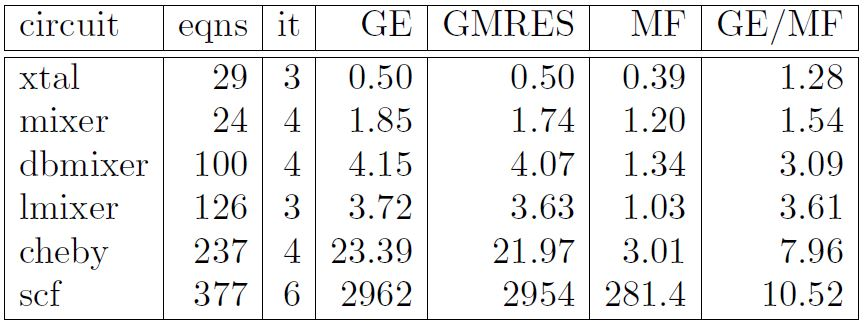
\includegraphics[width=.75\linewidth]{Tabella1.JPG}
    \caption{Comparazione\footnotemark di metodi diversi per la risoluzione dei circuiti elettronici.}
%    \label{fig:my_label}
\end{figure}
%Se la figura ha un'etichetta la si può usare per fare riferimento
%alla figura nel testo : Figura~\ref{fig:my_label}
\footnotetext{Risultati ottenuti con HP712/80 workstation.}
\end{frame}


\begin{frame} \frametitle{Matrix Free GMRES}
\begin{figure}
    \centering
    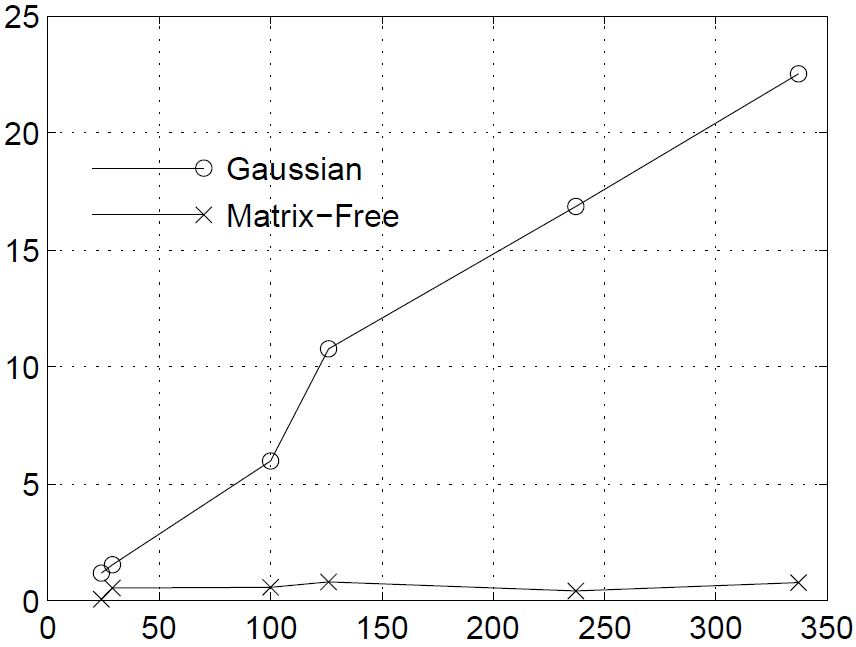
\includegraphics[width=.75\linewidth]{Figura1.JPG}
    \caption{Rapporto tra lo "shooting update time" e il costo di elaborazione del calcolo di una singola operazione.}
\end{figure}

\end{frame}


\begin{frame} \frametitle{Matrix Free GMRES}
\begin{figure}
    \centering
    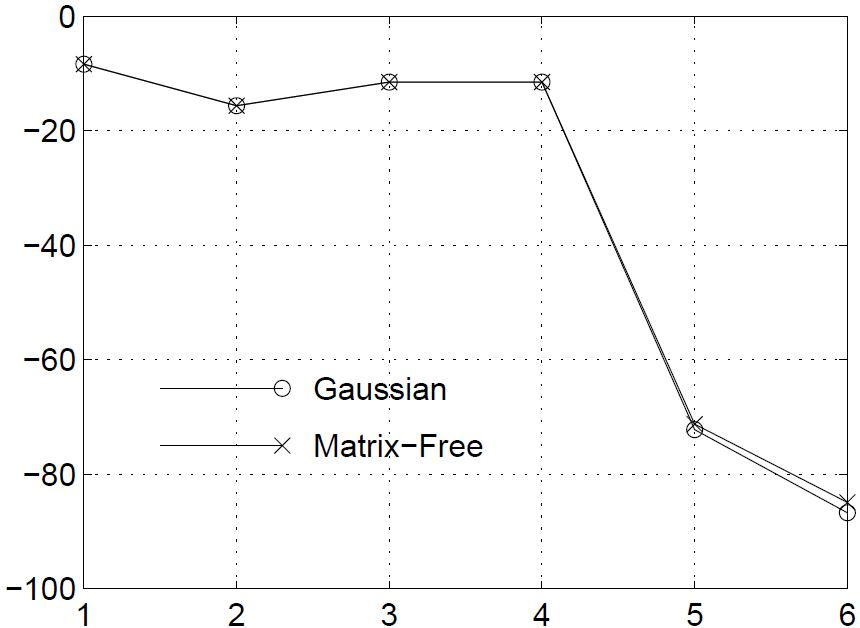
\includegraphics[width=.75\linewidth]{Figura2.JPG}
    \caption{Il grado di convergenza del metodo di Newton comparato al metodo Matrix Free.}
\end{figure}
\end{frame}


\begin{frame} \frametitle{Come inserire una formula}
Una formula può essere inserita all'interno del testo così : 
$-\nabla \left( \varepsilon \nabla u \right) = f $ oppure 
centrata e numerata così:
\begin{equation}\label{eq:poisson}
    -\nabla \cdot \left( \varepsilon \nabla u \right) = f
\end{equation}
oppure centrata senza numerazione così :
$$
 -\nabla \cdot \left( \varepsilon \nabla u \right) = f
$$
Posso fare riferimento alle formule numerate così : \eqref{eq:poisson}
\end{frame}

\begin{frame} \frametitle{Come inserire una lista per punti}
Ecco come inserire una lista per puti
\begin{itemize}
    \item un punto
    \item un altro
\end{itemize}
oppure un elenco numerato
\begin{enumerate}
    \item primo punto
    \item secondo punto
\end{enumerate}

\end{frame}



\begin{frame} \frametitle{Come inserire un pezzo di codice}
Si può evidenziare \alert{parte del testo} in questo modo.
%
Si può inserire un comando matlab all'interno del testo
in questo modo : \lstinline[language=Matlab]{for i = 1 : 10, disp (i), end}

si può inserire un un file contenete un codice matlab in questo modo :
\lstinputlisting[language=Matlab]{codice.m}

Si possono inserire solo alcune righe del file in questo modo :
\lstinputlisting[language=Matlab, firstline=1, lastline=2]{codice.m}

\end{frame}



\begin{frame} \frametitle{Come inserire una figura}
Questo è un esempio di come inserire una figura
\begin{figure}
    \centering
    \includegraphics[width=.75\linewidth]{iv.pdf}
    \caption{Questa è la didascalia}
    \label{fig:my_label}
\end{figure}
Se la figura ha un'etichetta la si può usare per fare riferimento
alla figura nel testo : Figura~\ref{fig:my_label}
\end{frame}

\begin{frame} \frametitle{Altra documentazione}
Questo è un esempio di come inserire un link ad un URL
\begin{itemize}
    \item Altre informazioni utili
    \begin{itemize}
        \item Il sito del \href{https://www.latex-project.org}{\LaTeX{}--project}
            \begin{itemize}
                \item Una lista di 
                \href{https://www.latex-project.org/get}{software offline ed online}\\
                per creare documenti \LaTeX{}
            \end{itemize}
        \item Un \href{https://en.wikibooks.org/wiki/LaTeX}{Wikibook} su \LaTeX
        \begin{itemize}
            \item La sezione sulle \href{https://en.wikibooks.org/wiki/LaTeX/Presentations}
            {presentazioni}
            \item La sezione sulle
            \href{https://en.wikibooks.org/wiki/LaTeX/Mathematics}{formule}
        \end{itemize}
        \item Un \href{https://tex.stackexchange.com/}{forum} con domande e risposte
        \item La documentazione di \href{https://it.overleaf.com/learn}{overleaf}
        \begin{itemize}
            \item Un \href{https://it.overleaf.com/learn/latex/Learn_LaTeX_in_30_minutes}
            {tutorial} per iniziare in 30 minuti
        \end{itemize}
        \item Uno strumento per \href{http://detexify.kirelabs.org/classify.html}
        {cercare simboli}
    \end{itemize}
\end{itemize}
\end{frame}
\end{document}
